\chapter{METODOLOGI}
\label{chap:metodologi}

% Ubah bagian-bagian berikut dengan isi dari desain dan implementasi

Penelitian ini dilaksanakan sesuai dengan desain sistem berikut ini beserta implementasinya. Desain sistem merupakan konsep dari pembuatan dan perencangan infrastruktur dan kemudian diwujudkan dalam bentuk blok-blok alur yang harus dikerjakan.

\section{Deskripsi Sistem}
\label{sec:deskripsisistem}

Tugas akhir ini merupakan penelitian yang mengintegrasikan teknologi visi komputer agar dapat mengontrol gerak kursi roda. Secara umum penelitian kali ini akan menggunakan desain sistem sesuai dengan Gambar \ref{fig:Metodologi Penelitian}.

% Gambar 3.1
\begin{figure} [ht] \centering
    % Nama dari file gambar yang diinputkan
    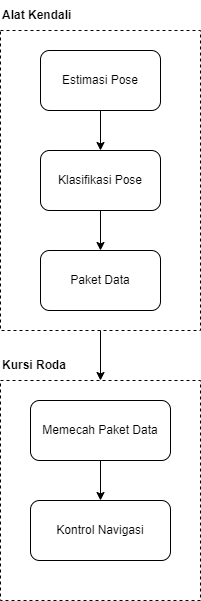
\includegraphics[scale=0.68]{gambar/blokDiagram.png}
    % Keterangan gambar yang diinputkan
    \caption{Blok Diagram Penelitian}
    % Label referensi dari gambar yang diinputkan
    \label{fig:Metodologi Penelitian}
\end{figure}

\subsection{Estimasi Pose}
Deteksi pose merupakan suatu proses yang melibatkan penggunaan bahasa pemrograman Python bersama dengan \emph{library} OpenCV dan \emph{framework} Mediapipe. Dalam konteks ini, Mediapipe berperan penting dalam mendapatkan informasi titik-titik \emph{landmark} yang signifikan pada objek yang diidentifikasi. \emph{Landmark} ini kemudian menjadi dasar untuk membentuk suatu representasi visual yang memvisualisasikan pose tersebut. Proses selanjutnya melibatkan penghubungan titik-titik \emph{landmark} yang telah ditentukan, di mana garis-garis dibuat untuk menggambarkan relasi spasial antar titik-titik tersebut. Dengan demikian, prosedur ini tidak hanya mengandalkan Mediapipe sebagai \emph{framework} utama, tetapi juga memanfaatkan OpenCV sebagai alat bantu untuk analisis citra dan manipulasi visual yang diperlukan dalam deteksi pose.

Pada penelitian kali ini akan memanfaatkan teknologi \emph{hand pose} dari Mediapipe untuk mengontrol gerak kursi roda. Terdapat beberapa titik \emph{keypoints} yang akan digunakan pada estimasi pose ini. Titik \emph{keypoints} yang akan digunakan pada estimasi  pose ini dapat dilihat pada Tabel \ref{tbl:titik keypoints}.

\begin{table}[H]
\centering
    \caption{Tabel titik \emph{keypoints} yang relevan pada tahap estimasi pose}
    \label{tbl:titik keypoints}
    \begin{tabular}{|c|c|}
        \hline
        Nomor Keypoint & Nama Keypoint      \\ \hline
        0              & Pergelangan Tangan \\ \hline
        1              & CMC Ibu Jari       \\ \hline
        2              & MPM Ibu Jari       \\ \hline
        3              & IP Ibu Jari        \\ \hline
        4              & TIP Ibu Jari       \\ \hline
        5              & MCP Telunjuk       \\ \hline
        6              & PIP Telunjuk       \\ \hline
        7              & DIP Telunjuk       \\ \hline
        8              & TIP Telunjuk       \\ \hline
        9              & MCP Jari Tengah    \\ \hline
        10             & PIP Jari Tengah    \\ \hline
        11             & DIP Jari Tengah    \\ \hline
        12             & TIP Jari Tengah    \\ \hline
        13             & MCP Jari Manis     \\ \hline
        14             & PIP Jari Manis     \\ \hline
        15             & DIP Jari Manis     \\ \hline
        16             & TIP Jari Manis     \\ \hline
        17             & MCP Kelingking     \\ \hline
        18             & PIP Kelingking     \\ \hline
        19             & DIP Kelingking     \\ \hline
        20             & TIP Kelingking     \\ \hline
    \end{tabular}
\end{table}

Setiap titik \emph{landmark} yang terdapat pada peraga akan diwarnai dengan warna yang unik untuk membedakan setiap jarinya. Secara spesifik, warna yang diberikan pada setiap titik \emph{landmark} mencerminkan asosiasi dengan jari tertentu, sehingga menciptakan representasi visual yang lebih terperinci dan informatif. Untuk memberikan gambaran yang lebih konkret maka berikut ini contoh citra yang telah diestimasi pose yang dapat dilihat pada Gambar \ref{fig:contoh citra yang telah diestimasi pose}.

% Gambar 3.2
\begin{figure} [ht] \centering
    % Nama dari file gambar yang diinputkan
    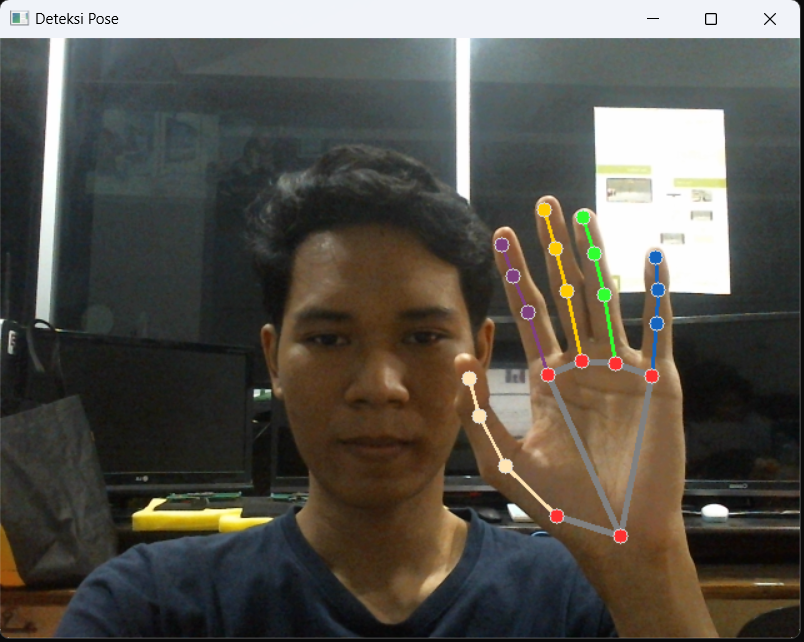
\includegraphics[scale=0.9]{gambar/bab3/EstimasiPose.png}
    % Keterangan gambar yang diinputkan
    \caption{Contoh citra yang telah diestimasi pose}
    % Label referensi dari gambar yang diinputkan
    \label{fig:contoh citra yang telah diestimasi pose}
\end{figure}

\subsection{Klasifikasi Pose}
Setelah proses estimasi pose tangan selesai, maka langkah selanjutnya ada mengelompokkan citra-citra hasil estimasi menjadi suatu dataset. Dataset ini akan memiliki 5 kelas berbeda yang masing-masing merepresentasikan perintah untuk maju, mundur, bergerak ke kanan, bergerak ke kiri, dan berhenti. Kelas ini mewakili perintah dasar untuk menggerakkan kursi roda. 

Untuk meningkatkan kinerja dan akurasi maka dataset ini kemudian akan melewati proses \emph{training} menggunakan algoritma \emph{Convolutional Neural Network} (CNN). Penggunaan CNN dalam \emph{training} dataset diharapkan dapat menghasilkan model yang mampu mengenali pola dan fitur yang kompleks, sehingga memungkinkan sistem untuk merespon dengan tepat terhadap variasi perintah yang mungkin diberikan oleh peraga. Hasil dari model prediksi yang telah dibuat dapat dilihat pada Tabel \ref{tbl:contoh-klasifikasi}.

\newpage

% Tabel 3.2
\begin{table}[H]
\centering
    \caption{Tabel contoh klasifikasi citra}
    \label{tbl:contoh-klasifikasi}
    \begin{tabular}{|c|c|}
        \hline
        Pose                & Citra              \\ \hline
        Kiri                & 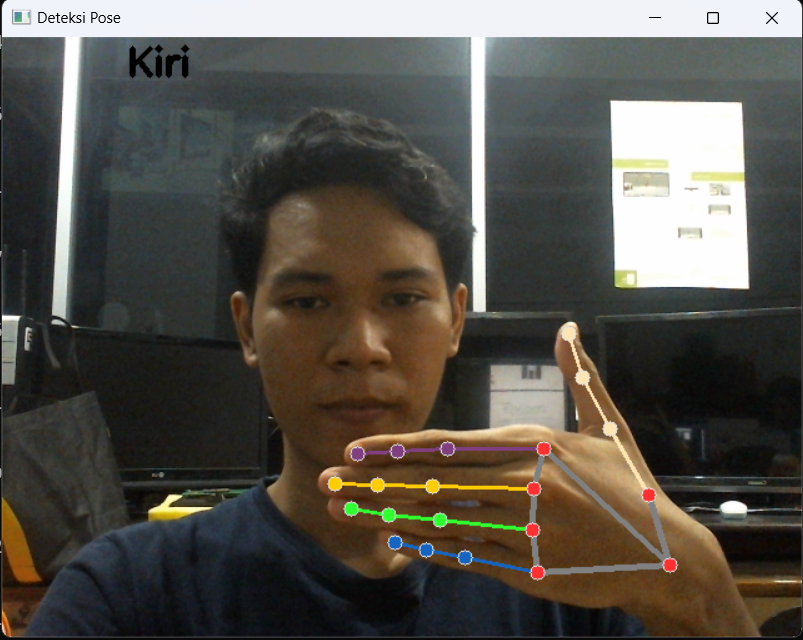
\includegraphics[scale=0.33]{gambar/bab3/Kiri.png}   \\ \hline
        Maju                & 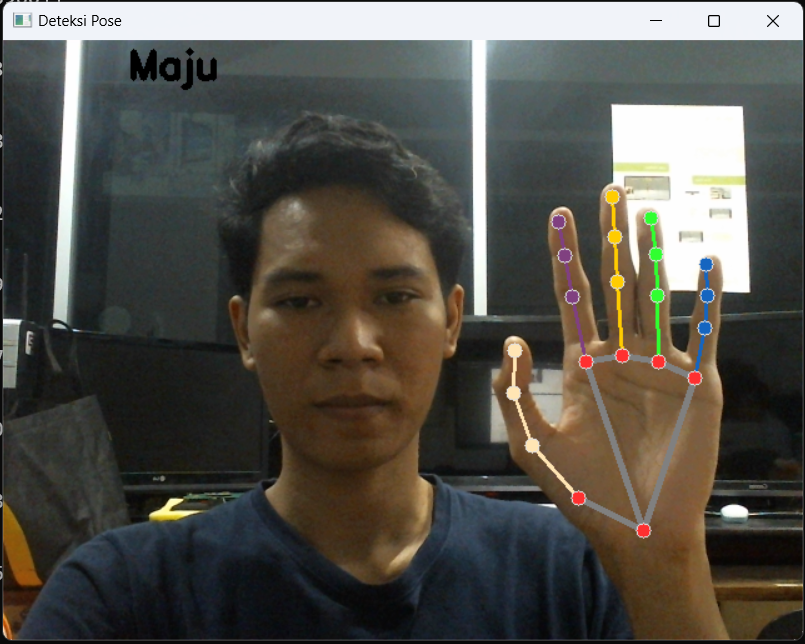
\includegraphics[scale=0.33]{gambar/bab3/Maju.png}   \\ \hline
        Stop                & 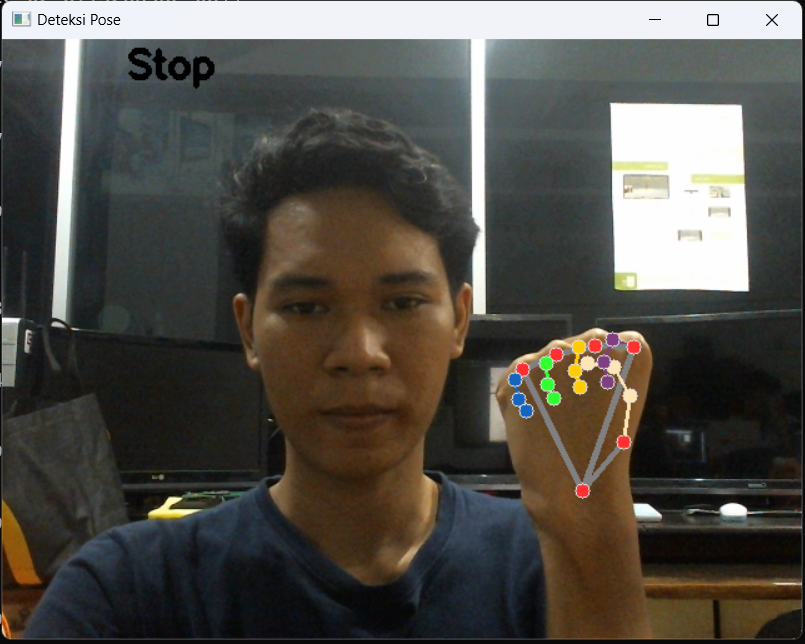
\includegraphics[scale=0.33]{gambar/bab3/Stop.png}   \\ \hline
        Mundur              & 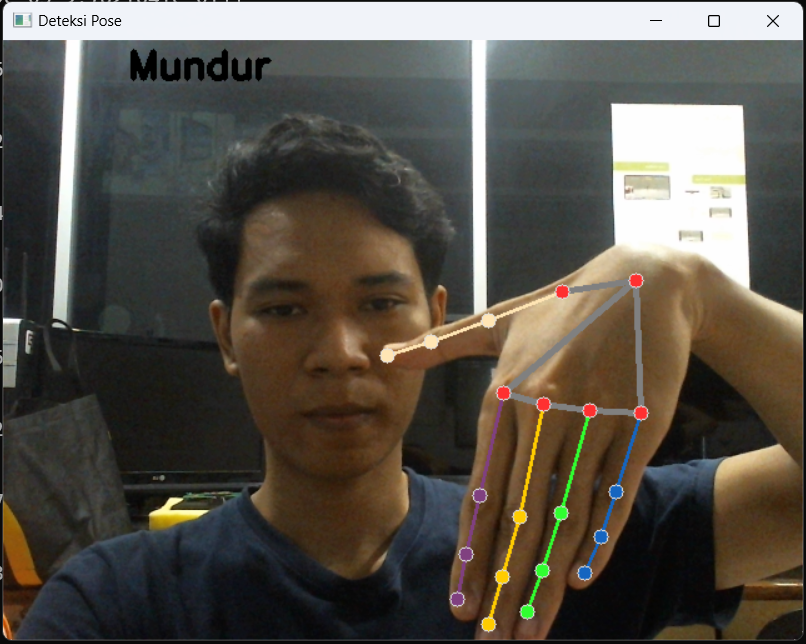
\includegraphics[scale=0.33]{gambar/bab3/Mundur.png} \\ \hline
        Kanan               & 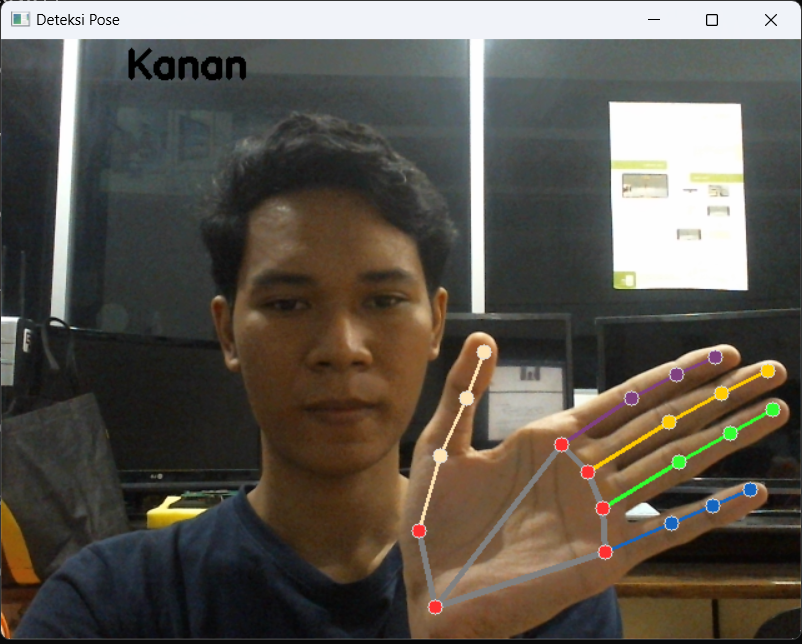
\includegraphics[scale=0.33]{gambar/bab3/Kanan.png}  \\ \hline
    \end{tabular}
\end{table}

\subsection{Paket Data}
Untuk dapat menggerakkan kursi roda maka perlu mengirimkan perintah ke kontroler kursi roda. Pada tahap klasifikasi pose telah didapatkan perintah dasar untuk menggerakkan kursi roda, seperti maju, mundur, kanan, kiri, maupun stop. Perintah ini kemudian akan digabungkan dengan kecepatan maksimal menjadi satu \emph{command} atau paket data seperti yang dilihat pada Persamaan \ref{eq:paket-data}.

% Persamaan 3.1
\begin{equation}
  \label{eq:paket-data}
    Arah(char),Kecepatan(integer)
\end{equation}

Variabel arah memiliki tipe data \emph{char} yang akan menentukan gerak dari motor kursi roda, serta variabel kecepatan memiliki tipe data integer yang akan menentukan kecepatan maksimal dari kursi roda. Untuk memperkecil ukuran data maka kode instruksi untuk menentukan arah gerak menggunakan satu huruf untuk mewakili setiap gerakan. Kode instruksi dapat dilihat pada Tabel \ref{tbl:kode-instruksi}. 

% Tabel 3.2
\begin{table}[H]
\centering
    \caption{Kode instruksi dari hasil klasifikasi}
    \label{tbl:kode-instruksi}
    \begin{tabular}{|c|c|}
        \hline
        Klasifikasi Pose & Kode Instruksi \\ \hline
        Kiri             & A              \\ \hline
        Maju             & B              \\ \hline
        Stop             & C              \\ \hline
        Mundur           & D              \\ \hline
        Kanan            & E              \\ \hline
    \end{tabular}
\end{table}

Setelah kedua variabel tersebut digabungkan maka akan dikirim secara nirkabel, baik menggunakan Bluetooth maupun WiFi dari laptop atau Jetson Nano ke ESP32.

\subsection{Memecahkan Paket Data}
Paket data yang telah dikirimkan melalui laptop maupun Jetson Nano akan diterima oleh ESP32 menggunakan Bluetooth maupun WiFi. Saat diterima oleh ESP32, data tersebut akan menjalani serangkaian proses yang melibatkan pemecahan paket data dan penyesuaian sesuai dengan variabel yang telah ditentukan sebelumnya. Pemecahan paket data ini memungkinkan ESP32 untuk mendekomposisi informasi yang terkandung dalam setiap paket dan memastikan bahwa setiap variabel terpisah dengan akurat. Dengan demikian proses ini akan mengorganisir dan menyusun kembali informasi serta memastikan bahwa setiap variabel telah benar sesuai dengan nama variabel dan tipe data yang disediakan.

\subsection{Kontrol Navigasi}
Kedua variabel yang didapatkan dari pemecahan paket data akan diproses pada ESP32. Variabel arah akan berperan untuk menentukan arah gerak dari motor, sedangkan variabel kecepatan akan digunakan untuk menetapkan kecepatan maksimal dari pergerakan motor tersebut. Terdapat serangkaian logika \emph{if} berantai pada kontrol navigasi, dimana empat variabel dir akan menentukan arah putaran motor. Selain itu, nilai PWM maksimal dikonfigurasi dengan menggunakan variabel kecepatan sehingga pengguna dapat menyesuaikan kecepatan maksimal motor yang pengguna inginkan. Dengan demikian pada tahap ini ESP32 dapat secara efektif memproses data yang diterima melalui sistem nirkabel dan menghasilkan instruksi kontrol yang sesuai untuk menggerakkan kursi roda dengan arah dan kecepatan yang diinginkan.


\section{Implementasi Alat}
\label{sec:implementasi alat}

Pada penelitian ini dikembangkan suatu alat kontrol yang dapat menerima perintah melalui perangkat lain seperti laptop maupun Jetson Nano secara nirkabel. Pada sub bab ini akan dijabarkan implementasi dari alat yang dikembangkan pada penelitian ini.

\subsection{\emph{Hardware} dan \emph{Software} yang digunakan}
Berikut ini dijabarkan beberapa \emph{Hardware} dan juga \emph{Software} yang digunakan pada penelitian ini seperti berikut:
\begin{enumerate}[nosep]
    \item Anaconda Navigator
    \item Arduino IDE 
    \item Laptop 
    \item Jetson Nano
    \item Kamera
    \item ESP32 Devkit V1
    \item 2 Kontroller Motor
    \item 2 DC-DC Voltage Regulator
    \item 2 DC Motor
    \item Baterai 24V
\end{enumerate}

\subsection{Skematik Alat}
Skematik pada alat ini diilustrasikan secara rinci pada Gambar 3.3. Sistem ini menggunakan kamera yang dihubungkan dengan Laptop atau Jetson Nano sebagai perangkat utama dalam menangkap citra. Proses kerja dimulai saat kamera menangkap citra objek. Citra yang telah ditangkap ini lantas diproses oleh Laptop atau Jetson Nano. Di dalam sistem ini, model klasifikasi yang telah diprogram sebelumnya memainkan peran penting dalam menginterpretasikan data citra tersebut. Hasil dari proses klasifikasi ini sangat krusial karena menjadi dasar dalam penentuan kode instruksi yang akan diimplementasikan.

Kode instruksi tersebut kemudian akan dikombinasikan dengan parameter kecepatam maksimal yang sebelumnya telah ditetapkan oleh pemngguna. Gabungan dari kode instruksi dan parameter kecepatan ini akan menjadi satu paket data sebagai kontrol gerak kursi roda. Paket data ini kemudian akan ditransmisikan secara nirkabel, baik dengan Bluetooth maupun WiFi, ke modul ESP32 Devkit V1. 

ESP32 memiliki peranan penting dalam kontrol motor kursi roda. ESP32 akan digunakan sebagai pusat pengendalian yang menerima paket data yang telah dikirimkan oleh pengguna secara nirkabel. Kemudian ESP32 akan melakukan pemecahan paket data dan menyesuaikan data tersebut kedalam variabel-variabel yang telah ditentukan. Proses pemecahan paket data ini akan menghasilkan dua data utama yang kemudian akan diproses lebih lanjut oleh ESP32.

Variabel pertama merupakan variabel arah yang memiliki fungsi krusial untuk menentukan arah gerak kedua motor pada kursi roda. Variabel ini akan memastikan bahwa motor bergerak sesuai dengan arah yang diinginkan sesuai dengan data yang diterima. Selain itu terdapat variabel kecepatan yang digunakan untuk menetapkan kecepatan maksimal pergerakan motor.

Dalam implementasinya terdapat serangkaian logika \emph{if} berantai yang akan dijelaskan secara terperinci pada sub bab program. Sederhananya logika \emph{if} berantai ini memiliki peran yang penting dalam pengambilan keputusan baik arah dan kecepatan motor sesuai dengan data yang telah diterima. Hasil dari logika ini akan memberikan \emph{trigger} berupa tegangan 5V ataupun 0V. Tegangan ini kemudian akan mempengaruhi arah putar motor.

Selanjutnya variabel kecepatan akan digunakan untuk mengatur tingkat \emph{Pulse Width Modulation} pada kontroler motor. Pengaturan PWM ini sangatlah penting guna mengatur kecepatan putar motor. Dengan mengatur tingkat PWM maka kecepatan motor maksimal dapat disesuaikan sesuai dengan kebutuhan.


\section{Kode Program}
Pada sub bab ini akan dijabarkan kode program yang digunakan pada penelitian ini.

\subsection{Program Untuk Memeriksa MAC Address Pada ESP32}
Agar dapat terhubung dengan Bluetooth pada ESP32 maka kita harus mengetahui MAC Address dari ESP32. Berikut merupakan program untuk memeriksa MAC Address Pada ESP32 dapat dilihat pada Program \ref{lst:CekMAC}.

% Program 3.1 
\begin{lstlisting}[
    language=Arduino,
    caption={Program Untuk Memeriksa MAC Address Pada ESP32},
    label={lst:CekMAC}
]
#include <BluetoothSerial.h>
BluetoothSerial SerialBT;

void setup() {
  Serial.begin(115200);
  SerialBT.begin("ESP32_Haris"); // Bluetooth device name
  delay(1000);  // Give some time for the Bluetooth module to initialize
}

void loop() {
  // Get the ESP32 Bluetooth address
  uint8_t esp32Address[6];
  esp_efuse_mac_get_default(esp32Address);

  // Print the address in a readable format
  Serial.printf("ESP32 Bluetooth Address: %02X:%02X:%02X:%02X:%02X:%02X\n",
                esp32Address[0], esp32Address[1], esp32Address[2],
                esp32Address[3], esp32Address[4], esp32Address[5]);
}
    
\end{lstlisting}

Program ini menggunakan \emph{library} BluetoothSerial dari Henry Abrahamsen. \emph{Library} ini menyediakan fungsionalitas untuk mengontrol modul Bluetooth pada ESP32 \parencite{Abrahamsen_2023}. Selanjutnya akan dibuat objek SerialBT dari kelas BluetoothSerial. Objek ini digunakan untuk berkomunikasi melalui Bluetooth. 

Pada void setup() terdapat Serial.begin() yang digunakan untuk menginisialisasi komunikasi serial dengan kecepatan 115200 bps. Selanjutnya modul Bluetooth diinisialisasikan dengan nama perangkat ESP32\_Haris. Berikan delay selama 1 detik agar Bluetooth dapat diinisialisasikan dengan baik.

Array esp32Address dideklarasi pada awal fungsi void loop(). Array ini akan digunakan untuk menyimpan alamat dari Bluetooth ESP32. fungsi esp\_efuse\_mac\_get\_default() digunakan untuk mendapatkan alamat Bluetooth dan menyimpannya dalam array esp32Address \parencite{Systems_2023}. Alamat Bluetooth kemudian akan dicetak ke Serial Monitor menjadi bentuk yang dapat dibaca dengan menggunakan kode Serial.printf(). 

\subsection{Program Untuk Menerima Data String Melalui Bluetooth Pada ESP32}

Program ini dirancang untuk menerima data string melalui Bluetooth dan memisahkannya menjadi 2 bagian. Kemudian terdapat data yang dievaluasi untuk mengetahui apakah data tersebut sudah berubah menjadi integer. Berikut ini merupakan Program \ref{lst:ReceivedBluetooth} yang digunakan untuk menguji kemampuan ESP32 dalam menerima data string melalui bluetooth.

% Program 3.2
\begin{lstlisting}[
    language=Arduino,
    caption={Program Untuk Menerima Data String Melalui Bluetooth Pada ESP32},
    label={lst:ReceivedBluetooth}
]
#include <BluetoothSerial.h>
BluetoothSerial SerialBT;

int maxspeed;

void setup(){
  Serial.begin(115200);
  SerialBT.begin("ESP32_Haris");
}

void loop(){
  if (SerialBT.available()){
    String receivedData = SerialBT.readStringUntil('\n');

    String arah = receivedData.substring(0, receivedData.indexOf(','));
    String kecepatan = receivedData.substring(receivedData.indexOf(',') + 1);

    maxspeed = kecepatan.toInt();

    Serial.print("Arah : ");
    Serial.println(arah);
    Serial.print("Kecepatan : ");
    Serial.println(kecepatan);

    if(maxspeed < 20){
      Serial.println("TRUE");
    }
    else{
      Serial.println("FALSE");
    }
  }
}
    
\end{lstlisting}

Program ini menggunakan \emph{library} BluetoothSerial dari Henry Abrahamsen. \emph{Library} ini menyediakan fungsionalitas untuk menerima data melalui koneksi Bluetooth dan mengolahnya \parencite{Abrahamsen_2023}. Selanjutnya akan dibuat objek SerialBT dari kelas BluetoothSerial. Objek ini selanjutnya digunakan untuk berkomunikasi melalui Bluetooth. Terdapat juga variabel maxspeed yang dideklarasikan sebagai suatu variabel yang menyimpan nilai kecepatan maksimum bertipe data integer.

Pada void setup() terdapat Serial.begin() yang digunakan untuk menginisialisasi komunikasi serial dengan kecepatan 115200 bps. Selanjutnya modul Bluetooth diinisialisasikan dengan nama perangkat ESP32\_Haris.

Pada fungsi void loop() akan berjalan terus-menerus setelah fungsi void setup(). Pertama-tama akan diperiksa apakah terdapat data yang tersedia untuk dibaca dari koneksi Bluetooth dengan menggunakan SerialBT.available(). Apabila terdapat data yang diterima maka data tersebut akan dimasukkan kedalam variabel receivedData yang bertipe string dengan menggunakan fungsi SerialBT.readStringUntil(). Data tersebut akan dibaca hingga menemukan karakter \emph{newline} ('\textbackslash n'). Data kemudian akan dipisahkan menjadi arah dan kecepatan. arah akan memisahkan data sebelum koma (',') dari receivedData. kecepatan akan memisahkan data setelah (',') hingga akhir receivedData. Tipe data dari variabel kecepatan ini kemudian akan diubah menjadi integer dan nilai tersebut dimasukkan ke dalam variabel maxspeed. Kemudian nilai pada variabel arah dan kecepatan akan ditampilkan ke \emph{Serial Monitor}. fungsi \emph{if} ditambahkan untuk menguji apakah variabel maxspeed sudah bertipe integer. Apabila nilai maxspeed kurang dari 20 maka akan ditampilkan \emph{boolean} \emph{True}, apabila lebih dari atau sama dengan 20 maka akan menampilkan \emph{boolean} \emph{False}.

\subsection{Program Untuk Menerima Data JSON Melalui Bluetooth Pada ESP32}

Program ini dirancang untuk menerima data JSON melalui Bluetooth dan memisahkannya menjadi 2 bagian. Berikut merupakan program untuk menguji kemampuan ESP32 dalam menerima data JSON melalui Bluetooth yang dapat dilihat pada Program \ref{lst:ReceivedBluetoothJSON}. 

% Program 3.3
\begin{lstlisting}[
    language=Arduino,
    caption={Program Untuk Menerima Data JSON Melalui Bluetooth Pada ESP32},
    label={lst:ReceivedBluetoothJSON}
]
#include <BluetoothSerial.h>
#include <ArduinoJson.h>

BluetoothSerial SerialBT;

void setup() {
  Serial.begin(115200);
  SerialBT.begin("ESP32_Haris");
}

void loop() {
  if (SerialBT.available()) {
    // Read the incoming data
    String json_data = SerialBT.readStringUntil('\n');

    // Deserialize the JSON
    DynamicJsonDocument doc(1024);
    DeserializationError error = deserializeJson(doc, json_data);

    if (error) {
      Serial.println("Failed to parse JSON");
    } else {
      // Extract values from JSON
      const char* arah = doc["arah"];
      const char* kecepatan = doc["kecepatan"];

      // Perform actions based on the received data
      Serial.print("Received Arah: ");
      Serial.println(arah);
      Serial.print("Received Kecepatan: ");
      Serial.println(kecepatan);
    }
  }
}
    
\end{lstlisting}

Program ini menggunakan \emph{library} BluetoothSerial dari Henry Abrahamsen dan ArduinoJson dari Beno\^{\i}t Blanchon. \emph{Library} BluetoothSerial menyediakan fungsionalitas untuk menerima data melalui koneksi Bluetooth \parencite{Abrahamsen_2023}. Sedangkan \emph{library} ArduinoJson digunakan untuk menguraikan \emph{deserialize} data JSON yang diterima \parencite{blanchon2021mastering}. Selanjutnya akan dibuat objek SerialBT dari kelas BluetoothSerial. Objek ini akan digunakan untuk berkomunikasi melalui Bluetooth.

Pada void setup() terdapat Serial.begin() untuk menginisialisasi komunikasi serial dengan kecepatan 115200 bps. Selanjutnya modul Bluetooth diinisialisasi dengan nama perangkat ESP\_Haris.

Pada fungsi void loop() akan berjalan terus-menerus setelah fungsi void setup(). Pertama-tama akan diperiksa apakah terdapat data yang tersedia untuk dibaca dari koneksi Bluetooth dengan menggunakan SerialBT.available(). Kemudian data akan dibaca dari koneksi Bluetooth hingga terdapat karakter \emph{newline} ('\textbackslash n') dan menyimpannya dalam string json\_data. Objek DynamicJsonDocument selanjutnya akan dibuat dengan kapasitas 1024 byte yang berguna untuk menampung dokumen JSON yang akan diuraikan. Data JSON yang telah ditampung kemudian hasilnya disimpan dalam objek doc. Jika terdapat kesalahan dalam proses deserialisasi maka pesan kesalahan akan ditampilkan. Lalu terdapat fungsi \emph{if} yang digunakan untuk memberikan pesan \emph{"Failed to parse JSON"} apabila terdapat kesalahan pada proses deserialisasi. Apabila tidak terdapat kesalahan maka setiap nilai dari atribut JSON akan diekstrak dengan nama arah dan kecepatan serta menyimpannya dalam variabel bertipe string. Nilai yang diterima dari atribut JSON akan dicetak ke \emph{Serial Monitor}.


\subsection{Program Untuk Menerima Data String Melalui \emph{Access Point} WiFi Pada ESP32}

Program ini dirancang sebagai server WiFi yang dapat menerima data dari \emph{client} yang terhubung dan mengolahnya. Data yang diterima akan diproses dan dipisahkan menjadi 2 variabel, yaitu variabel arah dan kecepatan. Kemudian nilai dari variabel kecepatan akan dimasukkan ke variabel maxspeed dan tipe datanya dievaluasi. Berikut merupakan Program \ref{lst:ReceivedWiFi} yang digunakan untuk menerima data string melalui \emph{Access Point} WiFi pada ESP32.

% Program 3.4
\begin{lstlisting}[
    language=Arduino,
    caption={Program Untuk Menerima Data String Melalui \emph{Access Point} WiFi Pada ESP32},
    label={lst:ReceivedWiFi}
]
#include <WiFi.h>
#include <Arduino.h>

int maxspeed;

const char* ssid = "Haris-Access-Point";
const char* password = "123456789";

WiFiServer server(80);

void setup(){
  Serial.begin(115200);


  // Connect to Wi-Fi network with SSID and password
  Serial.print("Setting AP Access Point");
  // Remove the password parameter, if you want the AP (Access Point) to be open
  WiFi.softAP(ssid, password);
 
  IPAddress IP = WiFi.softAPIP();
  Serial.print("ESP32 AP IP Address : ");
  Serial.println(IP);

  // Start the server
  server.begin();
}

void loop(){
    // Check if a client has connected
  WiFiClient client = server.available();

  if (client) {
    //Serial.println("New client connected");
    
    // Read the data from the client
    while (client.connected()) {
      if (client.available()) {
    
        String receivedData = client.readStringUntil('\n');

        String arah = receivedData.substring(0, receivedData.indexOf(','));
        String kecepatan = receivedData.substring(receivedData.indexOf(',') + 1);

        maxspeed = kecepatan.toInt();

        Serial.print("Arah : ");
        Serial.println(arah);
        Serial.print("Kecepatan : ");
        Serial.println(kecepatan);

        if(maxspeed < 20){
          Serial.println("TRUE");
        }
        else{
          Serial.println("FALSE");
        }

      }
    }

    client.stop();

  }
}
\end{lstlisting}

Program ini menggunakan \emph{library} WiFi yang menyediakan fungsionalitas untuk mengonfigurasi dan mengelola koneksi WiFi pada ESP32. Selain itu \emph{library} Arduino juga digunakan pada program ini yang menyediakan fungsi-fungsi dasar untuk pemrograman mikrokontroler. Variabel maxspeed dideklarasikan sebagai variabel yang menyimpan nilai integer yang kemudian digunakan untuk menyimpan nilai kecepatan maksimum. Variabel ssid akan digunakan untuk menyimpan nama jaringan WiFi yang akan dibuat dan variabel \emph{password} akan menyimpan nilai \emph{password} dari WiFi Server yang dibuat. Kedua variabel ini sangat penting agar ESP32 dapat dikonfigurasikan sebagai \emph{Access Point}. Selanjutnya objek server dibuat dari kelas WiFiServer untuk menangani koneksi pada port 80.

Pada void setup() terdapat Serial.begin() untuk menginisialisasi komunikasi serial dengan kecepatan 115200 bps. Lalu mengonfigurasi ESP32 sebagai \emph{Access Point} sesuai dengan SSID dan \emph{password} yang telah ditentukan. Apabila \emph{Access Point} telah dikonfigurasi maka IP \emph{Address} dari ESP32 akan disimpan pada variabel IP dan dicetak ke \emph{Serial Monitor}. server.begin() digunakan untuk memulai server pada port 80.

Fungsi void loop() akan berjalan terus-menerus setelah fungsi void setup() dijalankan. Pada fungsi ini terdapat WiFiClient yang digunakan untuk menguji apakah terdapat \emph{client} yang terhubung ke server. Jika terdapat \emph{client} yang terhubung maka akan masuk ke fungsi \emph{if}. Data yang dikirimkan akan dibaca secara terus-menerus melalui fungsi \emph{while}. Data yang diterima akan dimasukkan ke variabel receivedData hingga \emph{client} mengirimkan karakter \emph{newline} ('\textbackslash n'). Data kemudian akan dipisahkan menjadi arah dan kecepatan. arah akan memisahkan data sebelum koma (',') dari receivedData. kecepatan akan memisahkan data setelah (',') hingga akhir receivedData. Tipe data dari variabel kecepatan ini kemudian akan diubah menjadi integer dan nilai tersebut dimasukkan ke dalam variabel maxspeed. Kemudian nilai pada variabel arah dan kecepatan akan ditampilkan ke \emph{Serial Monitor}. fungsi \emph{if} ditambahkan untuk menguji apakah variabel maxspeed sudah bertipe integer. Apabila nilai maxspeed kurang dari 20 maka akan ditampilkan \emph{boolean} \emph{True}, apabila lebih dari atau sama dengan 20 maka akan menampilkan \emph{boolean} \emph{False}. Lalu koneksi akan ditutup setelah selesai membaca data dari \emph{client}.

\subsection{Program Untuk Menerima Data JSON Melalui \emph{Access Point} WiFi Pada ESP32}

Program ini dirancang untuk menerima data JSON melalui WiFi. ESP32 berperan sebagai \emph{Access Point} WiFi yang dapat menerima data JSON dari \emph{client} dan mencetaknya ke dalam \emph{Serial Monitor}. Berikut merupakan Program \ref{lst:ReceivedWiFiJSON} yang digunakan untuk menerima data JSON melalui \emph{Access Point} WiFi pada ESP32.

% Program 3.5
\begin{lstlisting}[
    language=Arduino,
    caption={Program Untuk Menerima Data JSON Melalui Access Point WiFi Pada ESP32},
    label={lst:ReceivedWiFiJSON}
]
#include <WiFi.h>
#include <Arduino.h>
#include <ArduinoJson.h>

int maxspeed;

const char* ssid = "B300-Access-Point";
const char* password = "123456789";

WiFiServer server(80);

void setup(){
  Serial.begin(115200);


  // Connect to Wi-Fi network with SSID and password
  Serial.print("Setting AP (Access Point)");
  // Remove the password parameter, if you want the AP (Access Point) to be open
  WiFi.softAP(ssid, password);
 
  IPAddress IP = WiFi.softAPIP();
  Serial.print("ESP32 AP IP Address : ");
  Serial.println(IP);

  // Start the server
  server.begin();
}

void loop(){
    // Check if a client has connected
  WiFiClient client = server.available();

  if (client) {
    //Serial.println("New client connected");
    
    // Read the data from the client
    while (client.connected()) {
      if (client.available()) {
    
        String json_data = client.readStringUntil('\n');

        DynamicJsonDocument doc(1024);
        DeserializationError error = deserializeJson(doc, json_data);

        if(error){
          Serial.println("Failed to parse JSON");
        }
        else{
          const char* arah = doc["arah"];
          int kecepatan = doc["kecepatan"];

          Serial.print("Received Arah : ");
          Serial.print(arah);
          Serial.print("   Received Kecepatan : ");
          Serial.println(kecepatan);
        }
      }
    }

    client.stop();

  }
}
\end{lstlisting}

Program ini menggunakan \emph{library} WiFi yang menyediakan fungsionalitas untuk mengkonfigurasi dan mengelola koneksi WiFi pada ESP32. Selain itu \emph{library} Arduino juga digunakan pada program ini yang menyediakan fungsi-fungsi dasar untuk pemrograman mikrokontroler. \emph{Library} ArduinoJson dari Beno\^{\i}t Blanchon digunakan untuk mengolah data JSON. Variabel maxspeed yang dideklarasikan sebagai suatu variabel yang menyimpan nilai kecepatan maksimum yang diterima dari data JSON. Variabel ssid dan password digunakan untuk menyimpan nilai nama dan \emph{password} untuk \emph{access point} yang akan dibuat oleh ESP32. lalu objek server dari kelas WiFiServer dibuat untuk menangani koneksi pada port 80.

Pada void setup() terdapat Serial.begin() yang digunakan untuk menginisialisasi komunikasi serial dengan kecepatan 115200 bps. Selanjutnya \emph{access point} akan dibuat sesuai dengan ssid dan password yang telah ditentukan sebelumnya. IP \emph{Address} kemudian akan ditampilkan pada \emph{Serial Monitor}. Akhirnya server akan dimulai pada port 80.

Fungsi void loop() akan berjalan terus-menerus setelah fungsi void setup() dijalankan. ESP32 akan mencoba untuk menerima koneksi dari \emph{client} melalui fungsi server.available(). Jika terdapat \emph{client} yang terhubung maka ESP32 akan memeriksa apakah \emph{client} masih tetap terhubung. Jika terdapat data yang tersedia maka data akan dibaca hingga terdapat karakter \emph{newline}('\textbackslash n'). Selanjutnya objek doc akan dibuat dari kelas DynamicJsonDocument dengan kapasitas 1024 \emph{byte}. Data yang didapatkan kemudian akan dipecah dengan menggunakan fungsi deserializeJson.

Jika terjadi kesalahan saat mengurai JSON maka program akan mencetak pesan \emph{error}. Jika \emph{parsing} JSON berhasil dilakukan, maka nilai dari JSON akan diakses. Data JSON akan diurai dan disimpan kedalam variabel arah serta kecepatan. Selanjutnya program akan menampilkan variabel tersebut ke \emph{Serial Monitor}. Setelah data JSON selesai diproses maka koneksi dengan \emph{client} akan ditutup.

\subsection{Program Untuk Menguji Rangkaian Kontrol ESP32}

Program ini dirancang untuk menguji rangkaian kontrol ESP32. Kedua motor akan diuji dan dikendalikan melalui modul ESP32 dan driver motor H-Bridge. Berikut program \ref{lst:MotorTest} yang digunakan untuk menguji rangkaian kontrol ESP32.

% Program 3.6
\begin{lstlisting}[
    language=Arduino,
    caption={Program Untuk Menguji Rangkaian Kontrol Pada ESP32},
    label={lst:MotorTest}
]
#include <Arduino.h>

//Motor Kiri
#define pwmpin1 5
#define dir1  18
#define dir2  19

//Motor kanan
#define pwmpin2 25
#define dir3 32
#define dir4 33

#define pwmChannel1  0
#define pwmChannel2  1
#define freq  15000
#define res  8

int PWM1_DutyCycle = 0;
int maxspeed = 127;


void setup() {
  // put your setup code here, to run once:
  
  pinMode(dir1,OUTPUT);
  pinMode(dir2,OUTPUT);
  pinMode(dir3,OUTPUT);
  pinMode(dir4,OUTPUT);
  //pinMode(pwmpin,OUTPUT);

  ledcSetup(pwmChannel1, freq, res);
  ledcSetup(pwmChannel2, freq, res);

  ledcAttachPin(pwmpin1, pwmChannel1);
  ledcAttachPin(pwmpin2, pwmChannel2);

  //ledcWrite(pwmChannel, 127);
}

void loop() {
  // put your main code here, to run repeatedly:

//MAJU
  //SOFTSTART
  while(PWM1_DutyCycle < maxspeed)
  {
    digitalWrite(dir1, HIGH);
    digitalWrite(dir2, LOW);
    digitalWrite(dir3, HIGH);
    digitalWrite(dir4, LOW);
    ledcWrite(pwmChannel1, PWM1_DutyCycle++);
    ledcWrite(pwmChannel2, PWM1_DutyCycle++);
    delay(10);
  }
  delay(5000);
  
  //SOFTSTOP
  while(PWM1_DutyCycle > 0)
  {
    digitalWrite(dir1, HIGH);
    digitalWrite(dir2, LOW);
    digitalWrite(dir3, HIGH);
    digitalWrite(dir4, LOW);
    ledcWrite(pwmChannel1, PWM1_DutyCycle--);
    ledcWrite(pwmChannel2, PWM1_DutyCycle--);
    delay(10);

  }
  delay(1000);

//MUNDUR
  while(PWM1_DutyCycle < maxspeed)
  {
    digitalWrite(dir1, LOW);
    digitalWrite(dir2, HIGH);
    digitalWrite(dir3, LOW);
    digitalWrite(dir4, HIGH);
    ledcWrite(pwmChannel1, PWM1_DutyCycle++);
    ledcWrite(pwmChannel2, PWM1_DutyCycle++);
    delay(10);
  }
  delay(5000);
  
  //SOFTSTOP
  while(PWM1_DutyCycle > 0)
  {
    digitalWrite(dir1, LOW);
    digitalWrite(dir2, HIGH);
    digitalWrite(dir3, LOW);
    digitalWrite(dir4, HIGH);
    ledcWrite(pwmChannel1, PWM1_DutyCycle--);
    ledcWrite(pwmChannel2, PWM1_DutyCycle--);
    delay(10);

  }
  delay(1000);

//BELOK KANAN
 while(PWM1_DutyCycle < maxspeed)
  {
    digitalWrite(dir1, HIGH);
    digitalWrite(dir2, LOW);
    digitalWrite(dir3, LOW);
    digitalWrite(dir4, LOW);
    ledcWrite(pwmChannel1, PWM1_DutyCycle++);
    ledcWrite(pwmChannel2, PWM1_DutyCycle++);
    delay(10);
  }
  delay(5000);
  
  //SOFTSTOP
  while(PWM1_DutyCycle > 0)
  {
    digitalWrite(dir1, HIGH);
    digitalWrite(dir2, LOW);
    digitalWrite(dir3, LOW);
    digitalWrite(dir4, LOW);
    ledcWrite(pwmChannel1, PWM1_DutyCycle--);
    ledcWrite(pwmChannel2, PWM1_DutyCycle--);
    delay(10);

  }
  delay(1000);

//BELOK KIRI
 while(PWM1_DutyCycle < maxspeed)
  {
    digitalWrite(dir1, LOW);
    digitalWrite(dir2, LOW);
    digitalWrite(dir3, HIGH);
    digitalWrite(dir4, LOW);
    ledcWrite(pwmChannel1, PWM1_DutyCycle++);
    ledcWrite(pwmChannel2, PWM1_DutyCycle++);
    delay(10);
  }
  delay(5000);
  
  //SOFTSTOP
  while(PWM1_DutyCycle > 0)
  {
    digitalWrite(dir1, LOW);
    digitalWrite(dir2, LOW);
    digitalWrite(dir3, HIGH);
    digitalWrite(dir4, LOW);
    ledcWrite(pwmChannel1, PWM1_DutyCycle--);
    ledcWrite(pwmChannel2, PWM1_DutyCycle--);
    delay(10);

  }
  delay(1000);

//STOP
 while(PWM1_DutyCycle < maxspeed)
  {
    digitalWrite(dir1, LOW);
    digitalWrite(dir2, LOW);
    digitalWrite(dir3, LOW);
    digitalWrite(dir4, LOW);
    ledcWrite(pwmChannel1, PWM1_DutyCycle++);
    ledcWrite(pwmChannel2, PWM1_DutyCycle++);
    delay(10);
  }
  delay(5000);
  
  //SOFTSTOP
  while(PWM1_DutyCycle > 0)
  {
    digitalWrite(dir1, LOW);
    digitalWrite(dir2, LOW);
    digitalWrite(dir3, LOW);
    digitalWrite(dir4, LOW);
    ledcWrite(pwmChannel1, PWM1_DutyCycle--);
    ledcWrite(pwmChannel2, PWM1_DutyCycle--);
    delay(10);

  }
  delay(1000);
}
\end{lstlisting}

\emph{Library} Arduino digunakan pada program ini. \emph{Library} ini menyediakan berbagai fungsi-fungsi dasar untuk pemrograman mikrokontroler. pwmPin1, dir1, dan dir2 merupakan variabel untuk mengatur kerja dari motor kiri. pwmPin1 didefinisikan dengan nilai 5 yang kemudian akan terhubung dengan GPIO5 pada ESP32, dir1 didefinisikan dengan nilai 18 yang kemudian akan terhubung dengan GPIO18 pada ESP32, dan dir2 yang didefinisikan dengan nilai 19 yang kemudian akan terhubung dengan GPIO19 pada ESP32. Selanjutnya terdapat pwmPin2, dir3, dan dir4 yang merupakan variabel yang digunakan untuk mengatur kerja dari motor kanan. pwmPin2 didefinisikan dengan nilai 25 yang kemudian akan terhubung dengan GPIO25 pada ESP32, dir3 didefinisikan dengan nilai 32 yang kemudian akan terhubung dengan GPIO32 pada ESP32, dan dir4 yang didefinisikan dengan nilai 33 yang kemudian akan terhubung dengan GPIO33 pada ESP32. Lalu variabel pwmChannel1, pwmChannel2, freq, dan res dideklarasikan. pwmChannel1 dan pwmChannel2 merupakan nomor saluran PWM yang digunakan. Variabel freq merupakan frekuensi PWM yang diatur menjadi 15kHz untuk meminimalisir \emph{noise} pada motor ketika bekerja. Variabel res digunakan untuk mengatur resolusi dari PWM yang diatur menjadi 8-bit. Variabel PWM1\_DutyCycle akan menyimpan siklus tugas yang kemudian akan digunakan untuk mengendalikan kecepatan motor dan variabel maxspeed merupakan nilai dari kecepatan motor maksimal.

Terdapat fungsi void setup() yang dieksekusi satu kali pada saat program pertama kali dijalankan. Pada fungsi ini terdapat dir1, dir2, dir3, dan dir4 yang diatur sebagai pin \emph{output}. ledcSetup merupakan fungsi dari \emph{library} ledc yang digunakan untuk mengonfigurasi saluran PWM. Fungsi ini memerlukan 3 variabel, yaitu pwmChannel, freq, dan res. Selanjutnya terdapat fungsi ledcAttachPin yang merupakan fungsi dari \emph{library} ledc yang digunakan untuk menghubungkan suatu pin dengan saluran PWM tertentu. Fungsi ini memerlukan 2 variabel, yaitu pin PWM dan juga PWM Channel. Secara keseluruhan, blok kode ini digunakan untuk melakukan konfigurasi pin-pin pada mikrokontroler ESP32 sehingga motor dapat dikendalikan. Pin-pin yang diatur sebagai \emph{output} akan digunakan tunuk mengatur arah putar motor. Sedangkan saluran PWM akan digunakan untuk mengatur kecepatan motor.

Pada fungsi void loop() terdapat serangkaian perintah yang mengatur gerakan kursi roda dengan menggunakan motor DC. Gerakan ini akan diulang secara terus-menerus. Hal ini berguna untuk menguji rangkaian kontrol pada ESP32. Setiap gerakan diawali dengan \emph{softstart} dan diakhiri dengan \emph{softstop}. Pada gerakan maju, kedua motor akan bergerak maju. Selama nilai PWM1\_DutyCycle kurang dari maxspeed, maka nilai PWM1\_DutyCycle akan ditambahkan secara bertahap hingga mencapai nilai maxspeed yang telah ditentukan. Selama itu juga kecepatan putar motor akan bertambah secara bertahap. Penambahan nilai PWM1\_DutyCycle akan ditunda selama 10 milidetik. Setelah PWM1\_DutyCycle mencapai nilai maxspeed maka kode selanjutnya akan ditunda selama 5 detik yang mengakibatkan motor akan berputar maju dengan kecepatan maksimum selama 5 detik. Setelah 5 detik, apabila nilai dari PWM1\_DutyCycle lebih dari 0 maka akan dilakukan \emph{softstop}. Arah putar kedua motor tetap diatur maju. Nilai PWM1\_DutyCycle akan diturunkan secara bertahap. Pengurangan nilai PWM1\_DutyCycle akan ditunda selama 10 milidetik. Apabila nilai PWM1\_DutyCycle sudah mencapai nilai 0 maka kode selanjutnya akan ditunda selama 1 detik. Langkah yang serupa akan dilakukan untuk setiap gerakan. Setiap gerakan memiliki fase \emph{softstart} dan \emph{softstop} yang bertujuan untuk memberikan perubahan kecepatan yang halus dan menghindari perubahan secara tiba-tiba. Penggunaan variabel PWM1\_DutyCycle digunakan untuk mengatur siklus kerja PWM untuk sebagai kontrol kecepatan yang fleksibel. fungsi \emph{delay} digunakan untuk memberikan jeda waktu antara setiap gerakan untuk mengatur durasi gerakan dan memberikan waktu bagi motor kursi roda untuk menyelesaikan setiap gerakan sebelum beralih ke gerakan berikutnya. Pada fungsi mundur, kedua roda akan berputar mundur. Pada fungsi belok kanan, roda kiri akan berputar maju sedangkan roda kanan tidak berputar sehingga kursi roda dapat berbelok ke arah kanan. Pada fungsi belok kiri, motor kiri tidak berputar namun roda kanan akan berputar maju sehingga kursi roda dapat berbelok ke arah kiri. Pada fungsi stop, kedua roda tidak akan berputar. Proses ini terus berulang didalam \emph{loop}, sehingga kursi roda akan melakukan gerakan berulang sesuai dengan logika yang telah diatur.


\subsection{Program Kontrol Motor Kursi Roda Melalui Bluetooth}
\begin{lstlisting}[
  language=Arduino,
  caption={Program Kontrol Motor Kursi Roda Melalui Bluetooth},
  label={lst:MotorBluetooth}
]
#include <BluetoothSerial.h>

#include <Arduino.h>

//Motor Kiri
#define pwmpin1 5
#define dir1 18
#define dir2 19

//Motor kanan
#define pwmpin2 25
#define dir3 32
#define dir4 33

//STATE Motor
int stdir[4];

#define pwmChannel1 0
#define pwmChannel2 1
#define freq 15000
#define res 8

int PWM1_DutyCycle = 0;
int maxspeed = 0;
int turnspeed = 0;

BluetoothSerial SerialBT;

void setup() {
  Serial.begin(115200);
  SerialBT.begin("ESP32_B300");

  pinMode(dir1, OUTPUT);
  pinMode(dir2, OUTPUT);
  pinMode(dir3, OUTPUT);
  pinMode(dir4, OUTPUT);

  ledcSetup(pwmChannel1, freq, res);
  ledcSetup(pwmChannel2, freq, res);

  ledcAttachPin(pwmpin1, pwmChannel1);
  ledcAttachPin(pwmpin2, pwmChannel2);

  Serial.begin(115200);

}

void loop() {
  if (SerialBT.available()) {
    String receivedData = SerialBT.readStringUntil('\n');

    String arah = receivedData.substring(0, receivedData.indexOf(','));
    String kecepatan = receivedData.substring(receivedData.indexOf(',') + 1);

    maxspeed = kecepatan.toInt();
    turnspeed = maxspeed / 2;

    Serial.print("Arah : ");
    Serial.println(arah);
    Serial.print("Kecepatan : ");
    Serial.println(kecepatan);

    if (arah == "A") {
      while (PWM1_DutyCycle <= turnspeed) {
        stdir[0] = LOW;
        stdir[1] = LOW;
        stdir[2] = HIGH;
        stdir[3] = LOW;

        digitalWrite(dir1, stdir[0]);
        digitalWrite(dir2, stdir[1]);
        digitalWrite(dir3, stdir[2]);
        digitalWrite(dir4, stdir[3]);
        ledcWrite(pwmChannel1, PWM1_DutyCycle++);
        ledcWrite(pwmChannel2, PWM1_DutyCycle++);
        delay(10);
      }

    } else if (arah == "B") {
      while (PWM1_DutyCycle <= maxspeed) {
        stdir[0] = HIGH;
        stdir[1] = LOW;
        stdir[2] = HIGH;
        stdir[3] = LOW;

        digitalWrite(dir1, stdir[0]);
        digitalWrite(dir2, stdir[1]);
        digitalWrite(dir3, stdir[2]);
        digitalWrite(dir4, stdir[3]);
        ledcWrite(pwmChannel1, PWM1_DutyCycle++);
        ledcWrite(pwmChannel2, PWM1_DutyCycle++);
        delay(10);
      }

    } else if (arah == "C") {
      while (PWM1_DutyCycle >= 0) {

        digitalWrite(dir1, stdir[0]);
        digitalWrite(dir2, stdir[1]);
        digitalWrite(dir3, stdir[2]);
        digitalWrite(dir4, stdir[3]);
        ledcWrite(pwmChannel1, PWM1_DutyCycle--);
        ledcWrite(pwmChannel2, PWM1_DutyCycle--);
        delay(10);
      }
    } else if (arah == "D") {
      while (PWM1_DutyCycle <= turnspeed) {
        stdir[0] = LOW;
        stdir[1] = HIGH;
        stdir[2] = LOW;
        stdir[3] = HIGH;

        digitalWrite(dir1, stdir[0]);
        digitalWrite(dir2, stdir[1]);
        digitalWrite(dir3, stdir[2]);
        digitalWrite(dir4, stdir[3]);
        ledcWrite(pwmChannel1, PWM1_DutyCycle++);
        ledcWrite(pwmChannel2, PWM1_DutyCycle++);
        delay(10);
      }

    } else if (arah == "E") {
      while (PWM1_DutyCycle <= turnspeed) {
        stdir[0] = HIGH;
        stdir[1] = LOW;
        stdir[2] = LOW;
        stdir[3] = LOW;

        digitalWrite(dir1, stdir[0]);
        digitalWrite(dir2, stdir[1]);
        digitalWrite(dir3, stdir[2]);
        digitalWrite(dir4, stdir[3]);
        ledcWrite(pwmChannel1, PWM1_DutyCycle++);
        ledcWrite(pwmChannel2, PWM1_DutyCycle++);
        delay(10);
      }

    }
  }
}  
\end{lstlisting}

\subsection{Program Kontrol Motor Kursi Roda Melalui \emph{Access Point} WiFi}
\begin{lstlisting}[
  language=Arduino,
  caption={Program Kontrol Motor Kursi Roda Melalui \emph{Access Point} WiFi},
  label={lst:MotorWiFiAP}
]
#include <WiFi.h>
#include <Arduino.h>

//WiFi Configuration
const char* ssid = "Haris-Access-Point";
const char* password = "123456789";

WiFiServer server(80);

//Motor Kiri
#define pwmpin1 5
#define dir1 18
#define dir2 19

//Motor kanan
#define pwmpin2 25
#define dir3 32
#define dir4 33

//STATE Motor
int stdir[4];

#define pwmChannel1 0
#define pwmChannel2 1
#define freq 15000
#define res 8

int PWM1_DutyCycle = 0;
int maxspeed = 70;
int turnspeed = 35;
int kecepatan = 0;

void setup() {
  Serial.begin(115200);
  Serial.print("Setting AP (Access Point) ...");
  WiFi.softAP(ssid, password);

  IPAddress IP = WiFi.softAPIP();
  Serial.print("ESP32 AP IP Address : ");
  Serial.println(IP);

  server.begin();

  pinMode(dir1, OUTPUT);
  pinMode(dir2, OUTPUT);
  pinMode(dir3, OUTPUT);
  pinMode(dir4, OUTPUT);

  ledcSetup(pwmChannel1, freq, res);
  ledcSetup(pwmChannel2, freq, res);

  ledcAttachPin(pwmpin1, pwmChannel1);
  ledcAttachPin(pwmpin2, pwmChannel2);

  Serial.begin(115200);

}

void loop() {
  WiFiClient client = server.available();
  if(client){
    while(client.connected()){
      if(client.available()){

        String arah = client.readStringUntil('\n');
        Serial.print("Arah : ");
        Serial.println(arah);

        if(arah == "A"){
          while(PWM1_DutyCycle <= turnspeed){
            stdir[0] = LOW;
            stdir[1] = LOW;
            stdir[2] = HIGH;
            stdir[3] = LOW;

            digitalWrite(dir1, stdir[0]);
            digitalWrite(dir2, stdir[1]);
            digitalWrite(dir3, stdir[2]);
            digitalWrite(dir4, stdir[3]);
            ledcWrite(pwmChannel1, PWM1_DutyCycle++);
            ledcWrite(pwmChannel2, PWM1_DutyCycle++);
            delay(10);
          }
        }
        else if(arah == "B"){
          while(PWM1_DutyCycle <= maxspeed){
            stdir[0] = HIGH;
            stdir[1] = LOW;
            stdir[2] = HIGH;
            stdir[3] = LOW;

            digitalWrite(dir1, stdir[0]);
            digitalWrite(dir2, stdir[1]);
            digitalWrite(dir3, stdir[2]);
            digitalWrite(dir4, stdir[3]);
            ledcWrite(pwmChannel1, PWM1_DutyCycle++);
            ledcWrite(pwmChannel2, PWM1_DutyCycle++);
            delay(10);
          }
        }
        else if(arah == "C"){
          while(PWM1_DutyCycle >= 0){
            digitalWrite(dir1, stdir[0]);
            digitalWrite(dir2, stdir[1]);
            digitalWrite(dir3, stdir[2]);
            digitalWrite(dir4, stdir[3]);
            ledcWrite(pwmChannel1, PWM1_DutyCycle--);
            ledcWrite(pwmChannel2, PWM1_DutyCycle--);
            delay(10);
          }
        }
        else if(arah == "D"){
          while(PWM1_DutyCycle <= turnspeed){
            stdir[0] = LOW;
            stdir[1] = HIGH;
            stdir[2] = LOW;
            stdir[3] = HIGH;

            digitalWrite(dir1, stdir[0]);
            digitalWrite(dir2, stdir[1]);
            digitalWrite(dir3, stdir[2]);
            digitalWrite(dir4, stdir[3]);
            ledcWrite(pwmChannel1, PWM1_DutyCycle++);
            ledcWrite(pwmChannel2, PWM1_DutyCycle++);
            delay(10);
          }
        }
        else if(arah == "E"){
          while(PWM1_DutyCycle <= turnspeed){
            stdir[0] = HIGH;
            stdir[1] = LOW;
            stdir[2] = LOW;
            stdir[3] = LOW;

            digitalWrite(dir1, stdir[0]);
            digitalWrite(dir2, stdir[1]);
            digitalWrite(dir3, stdir[2]);
            digitalWrite(dir4, stdir[3]);
            ledcWrite(pwmChannel1, PWM1_DutyCycle++);
            ledcWrite(pwmChannel2, PWM1_DutyCycle++);
            delay(10);
          }
        }
      }
    }
  }
}  
\end{lstlisting}

\subsection{Program Untuk Mengirim Data String Melalui Bluetooth}

% Program 3.7
\begin{lstlisting}[
    language=Python,
    caption={Program Untuk Mengirim Data String Melalui Bluetooth},
    label={lst:SendBluetooth}
]
import bluetooth
import datetime

# ESP32's Bluetooth MAC address
esp32_mac_address = "30:C6:F7:2F:31:86"  # Replace with your ESP32's MAC addres

# Establish a Bluetooth connection
sock = bluetooth.BluetoothSocket(bluetooth.RFCOMM)
sock.connect((esp32_mac_address, 1))  # Channel 1 is commonly used for SPP (Serial Port Profile)

while True:
    # Send two data values
    arah = input("Enter arah : ")
    kecepatan = input("Enter kecepatan : ")
    message = f"{arah},{kecepatan}"
    date = datetime.datetime.now()
    print(date)
    
    if arah == "q" or kecepatan == "q":
        break
    
    sock.send(message)

# Close the Bluetooth connection
sock.close()

\end{lstlisting}

\subsection{Program Untuk Mengirim Data String Melalui WiFi}

% Program 3.8
\begin{lstlisting}[
  language=Python,
  caption={Program Untuk Mengirim Data String Melalui WiFi},
  label={lst:SendWiFiAP}
]
import socket
import time

import datetime

host = "192.168.4.1" # Set to ESP32 Access Point IP Address
port = 80

# Create a socket connection
with socket.socket(socket.AF_INET, socket.SOCK_STREAM) as s:
    # Connect to the ESP32 server
    s.connect((host, port))
    
    while True:
        # Send two data values
        arah = input("Enter arah : ")
        kecepatan = input("Enter kecepatan : ")
        message = f"{arah},{kecepatan}"
        date = datetime.datetime.now()
        print(date)
    
        if arah == "q" or kecepatan == "q":
            break
    
        s.send(message.encode('utf-8'))
        
s.close()

\end{lstlisting}

\subsection{Program Untuk Mengirim Data JSON Melalui Bluetooth}

% Program 3.9
\begin{lstlisting}[
    language=Python,
    caption={Program Untuk Mengirim Data JSON Melalui Bluetooth},
    label={lst:SendBluetoothJSON}
]
import bluetooth
import json

# ESP32 Bluetooth address
esp32_address = "EC:62:60:9B:E4:92"  # Replace with your ESP32's Bluetooth address

# esp32_address = "30:C6:F7:2F:31:86" # Iqbal's ESP32

# Create a Bluetooth socket
sock = bluetooth.BluetoothSocket(bluetooth.RFCOMM)

# Connect to the ESP32
sock.connect((esp32_address, 1))

while True:
    # Get keyboard input for two values
    arah = input("Masukkan Arah: ")
    kecepatan = input("Masukkan Kecepatan: ")
    
    # Create a JSON object
    json_data = {"arah": arah, "kecepatan": kecepatan}

    # Serialize the JSON data
    json_string = json.dumps(json_data)
    
    if arah == "q" or kecepatan == "q":
        break

    # Send the serialized JSON over Bluetooth
    sock.send(json_string)

# Close the Bluetooth socket
sock.close()

\end{lstlisting}

\subsection{Program Untuk Mengirim Data JSON Melalui WiFi}

% Program 3.9
\begin{lstlisting}[
  language=Python,
  caption={Program Untuk Mengirim Data JSON Melalui WiFi},
  label={lst:SendWiFiJSON}
]
import socket
import time
import json

import datetime

host = "192.168.4.1" # Set to ESP32 Access Point IP Address
port = 80

# Create a socket connection
with socket.socket(socket.AF_INET, socket.SOCK_STREAM) as s:
    # Connect to the ESP32 server
    s.connect((host, port))
    
    while True:
        arah = input("Masukkan Arah: ")
        kecepatan = input("Masukkan Kecepatan: ")
        
        json_data = {"arah": arah, "kecepatan": kecepatan}
        date = datetime.datetime.now()
        
        if arah == q or kecepatan == q:
            break
        else:
            json_string = json.dumps(json_data)
            s.send(json_string.encode('utf-8'))
            print(f"{date} -> {json_data}")

s.close()
\end{lstlisting}
